\documentclass[12pt, openright, twoside]{report}
% Language and encoding
\usepackage[utf8]{inputenc}
\usepackage[english]{babel}
% Page layout and margins
\usepackage[a4paper, margin=1in]{geometry}
% Graphics and captions
\usepackage{graphicx}                 % For including images
\usepackage{subcaption}               % For subfigures (if needed)
\usepackage[labelfont=bf, figurename=Fig., tablename=Table, font=small]{caption}
\captionsetup{font={small, stretch=1.2}} 

% Math and symbols
\usepackage{amsmath} % For advanced math commands
\usepackage{amssymb} % For additional symbols
\usepackage{bbold}   % For bold mathematical symbols
% References
\usepackage[backend=biber, sorting=none]{biblatex} % For references
\addbibresource{references.bib}                     % Point to your bibliography file
% Title and section formatting
\usepackage{titlesec}
\titleformat{\section}{\normalfont\Large\bfseries}{\thesection}{1em}{}
\titleformat{\subsection}{\normalfont\large\bfseries}{\thesubsection}{1em}{}
% Lists and tables
\usepackage{enumitem} % For custom lists
\usepackage{multirow} % For tables with merged rows
\usepackage{multicol} % For multi-column text (if needed)
% Typography improvements
\usepackage{microtype} % Improves text justification and spacing
% Custom margins for specific content
\usepackage{changepage} % To change margins for specific sections (e.g., images)
% Floating objects
\usepackage{float} % For precise positioning of floats
% Miscellaneous
\usepackage{comment} % To comment out large blocks of text
% TikZ and PGFPlots (if needed for graphs)
\usepackage{tikz} % For custom graphics
\usepackage{pgfplots} % For plots and charts
\pgfplotsset{compat=1.18}
% Reduce compilation time (useful for TikZ-heavy documents)
\usepgfplotslibrary{external}
\tikzexternalize
% Line spacing
\renewcommand{\baselinestretch}{1.5}
% Headers and footers (if customization is needed)
\usepackage{fancyhdr}
\pagestyle{fancy}
% Configure the fancy header
\renewcommand{\headrulewidth}{0.4pt} % Adds a horizontal line
\fancyhead[C]{Martina Arrighini, Luigi Babiski Arruda, Giorgio Cottini, Enrico Paciaroni}
\fancyfoot[C]{\thepage}
% Hyperlinks
\usepackage{hyperref}
\hypersetup{
    colorlinks=true,
    linkcolor=blue,
    filecolor=magenta,
    urlcolor=cyan,
    pdftitle={Group Project Report},
    pdfpagemode=FullScreen,
}

\begin{document}

%-------- Title page -------------------------------------------------------------------------------------------------------%

    \begin{titlepage}
        \centering
        
\includegraphics[width=0.3\textwidth]{images/logo_unipd.png}\par\vspace{1cm}
        {\scshape\LARGE Università degli Studi di Padova \par}
        \vspace{1.5cm}
        {\scshape\Large Master Degree Course in Computational Finance \par}
        \vspace{.2cm}
        {\scshape\large Regression and Time Series Models \par}
        \vspace{1.5cm}
        {\Large\bfseries Group Work 1 - Regression with CAPM Model\par}
        \vspace{1.5cm}
        {\itshape Martina Arrighini, 2149799, martina.arrighini@studenti.unipd.it \par}
        {\itshape Luigi Babiski Arruda, 2031997, luigi.babiskiarruda@studenti.unipd.it\par}
        {\itshape Giorgio Cottini, 2140740, giorgio.cottini@studenti.unipd.it \par}
        {\itshape Enrico Paciaroni, 2139678, enrico.paciaroni@studenti.unipd.it \par}
        \vfill
        Commissioned by: \par
        Prof.\ Massimiliano Caporin
        \vfill
        {\large A.Y. 2024/2025}
    \end{titlepage}

\setcounter{page}{1}

%-------- Assignment 1 -----------------------------------------------------------------------------------------------------%
\section*{Assignment 1}

%-------- Assignment 2 -----------------------------------------------------------------------------------------------------%
\section*{Assignment 2}
\begin{figure}[h!]
    \centering
    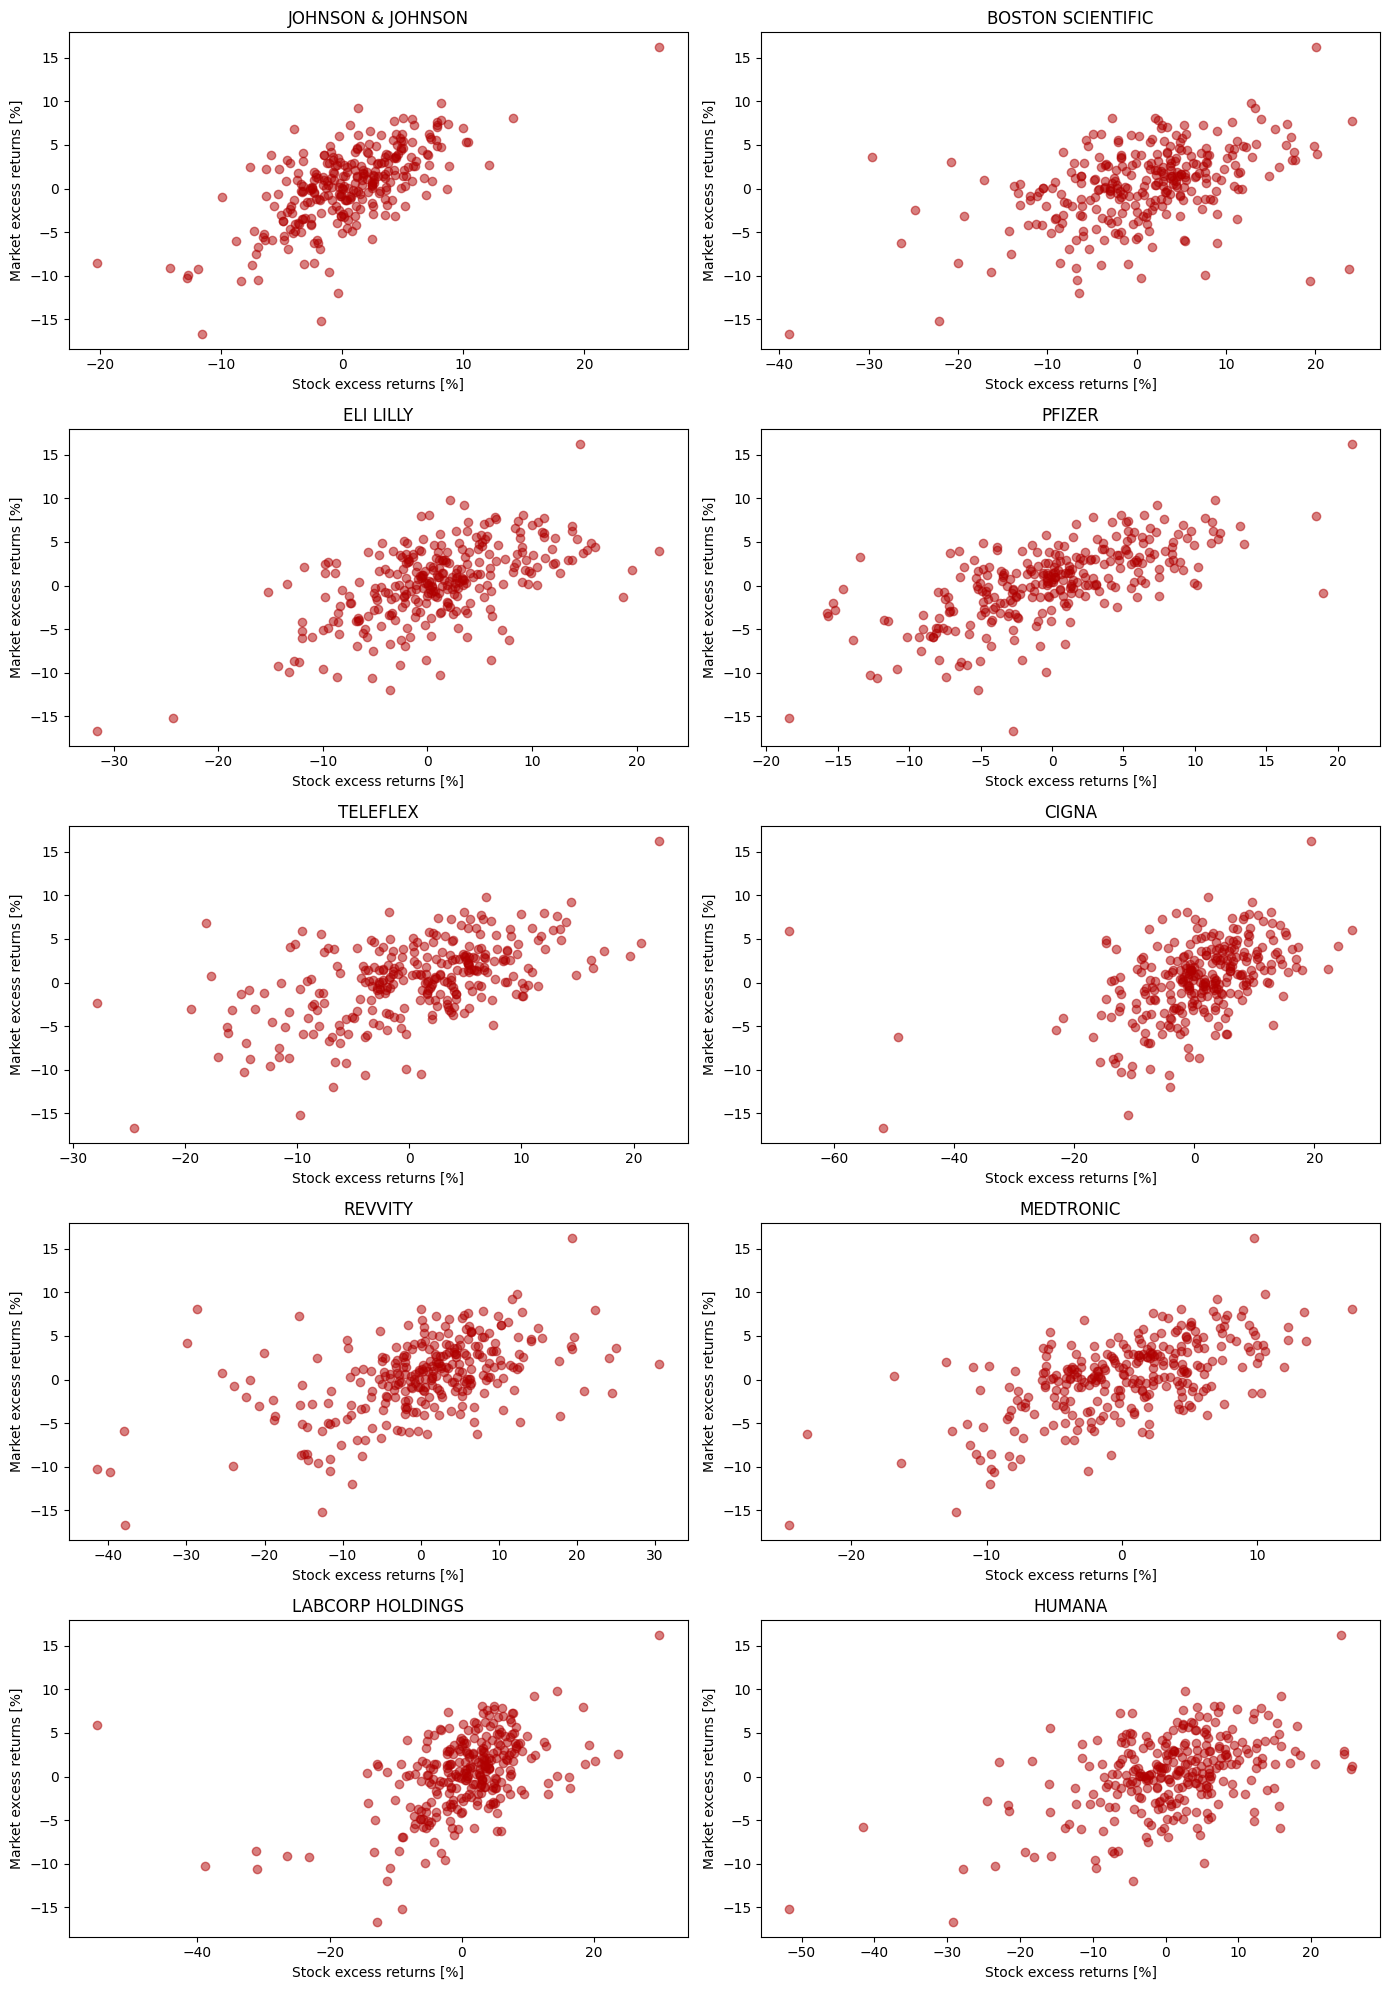
\includegraphics[width=0.9\textwidth]{images/equities_scatterplot.png}
    \caption{Scatterplot of equities' log-returns against excess market returns.}\label{fig:equities_scatterplot}
\end{figure}

%-------- Assignment 3 -----------------------------------------------------------------------------------------------------%
\section*{Assignment 3}
\begin{figure}[h!]
    \centering
    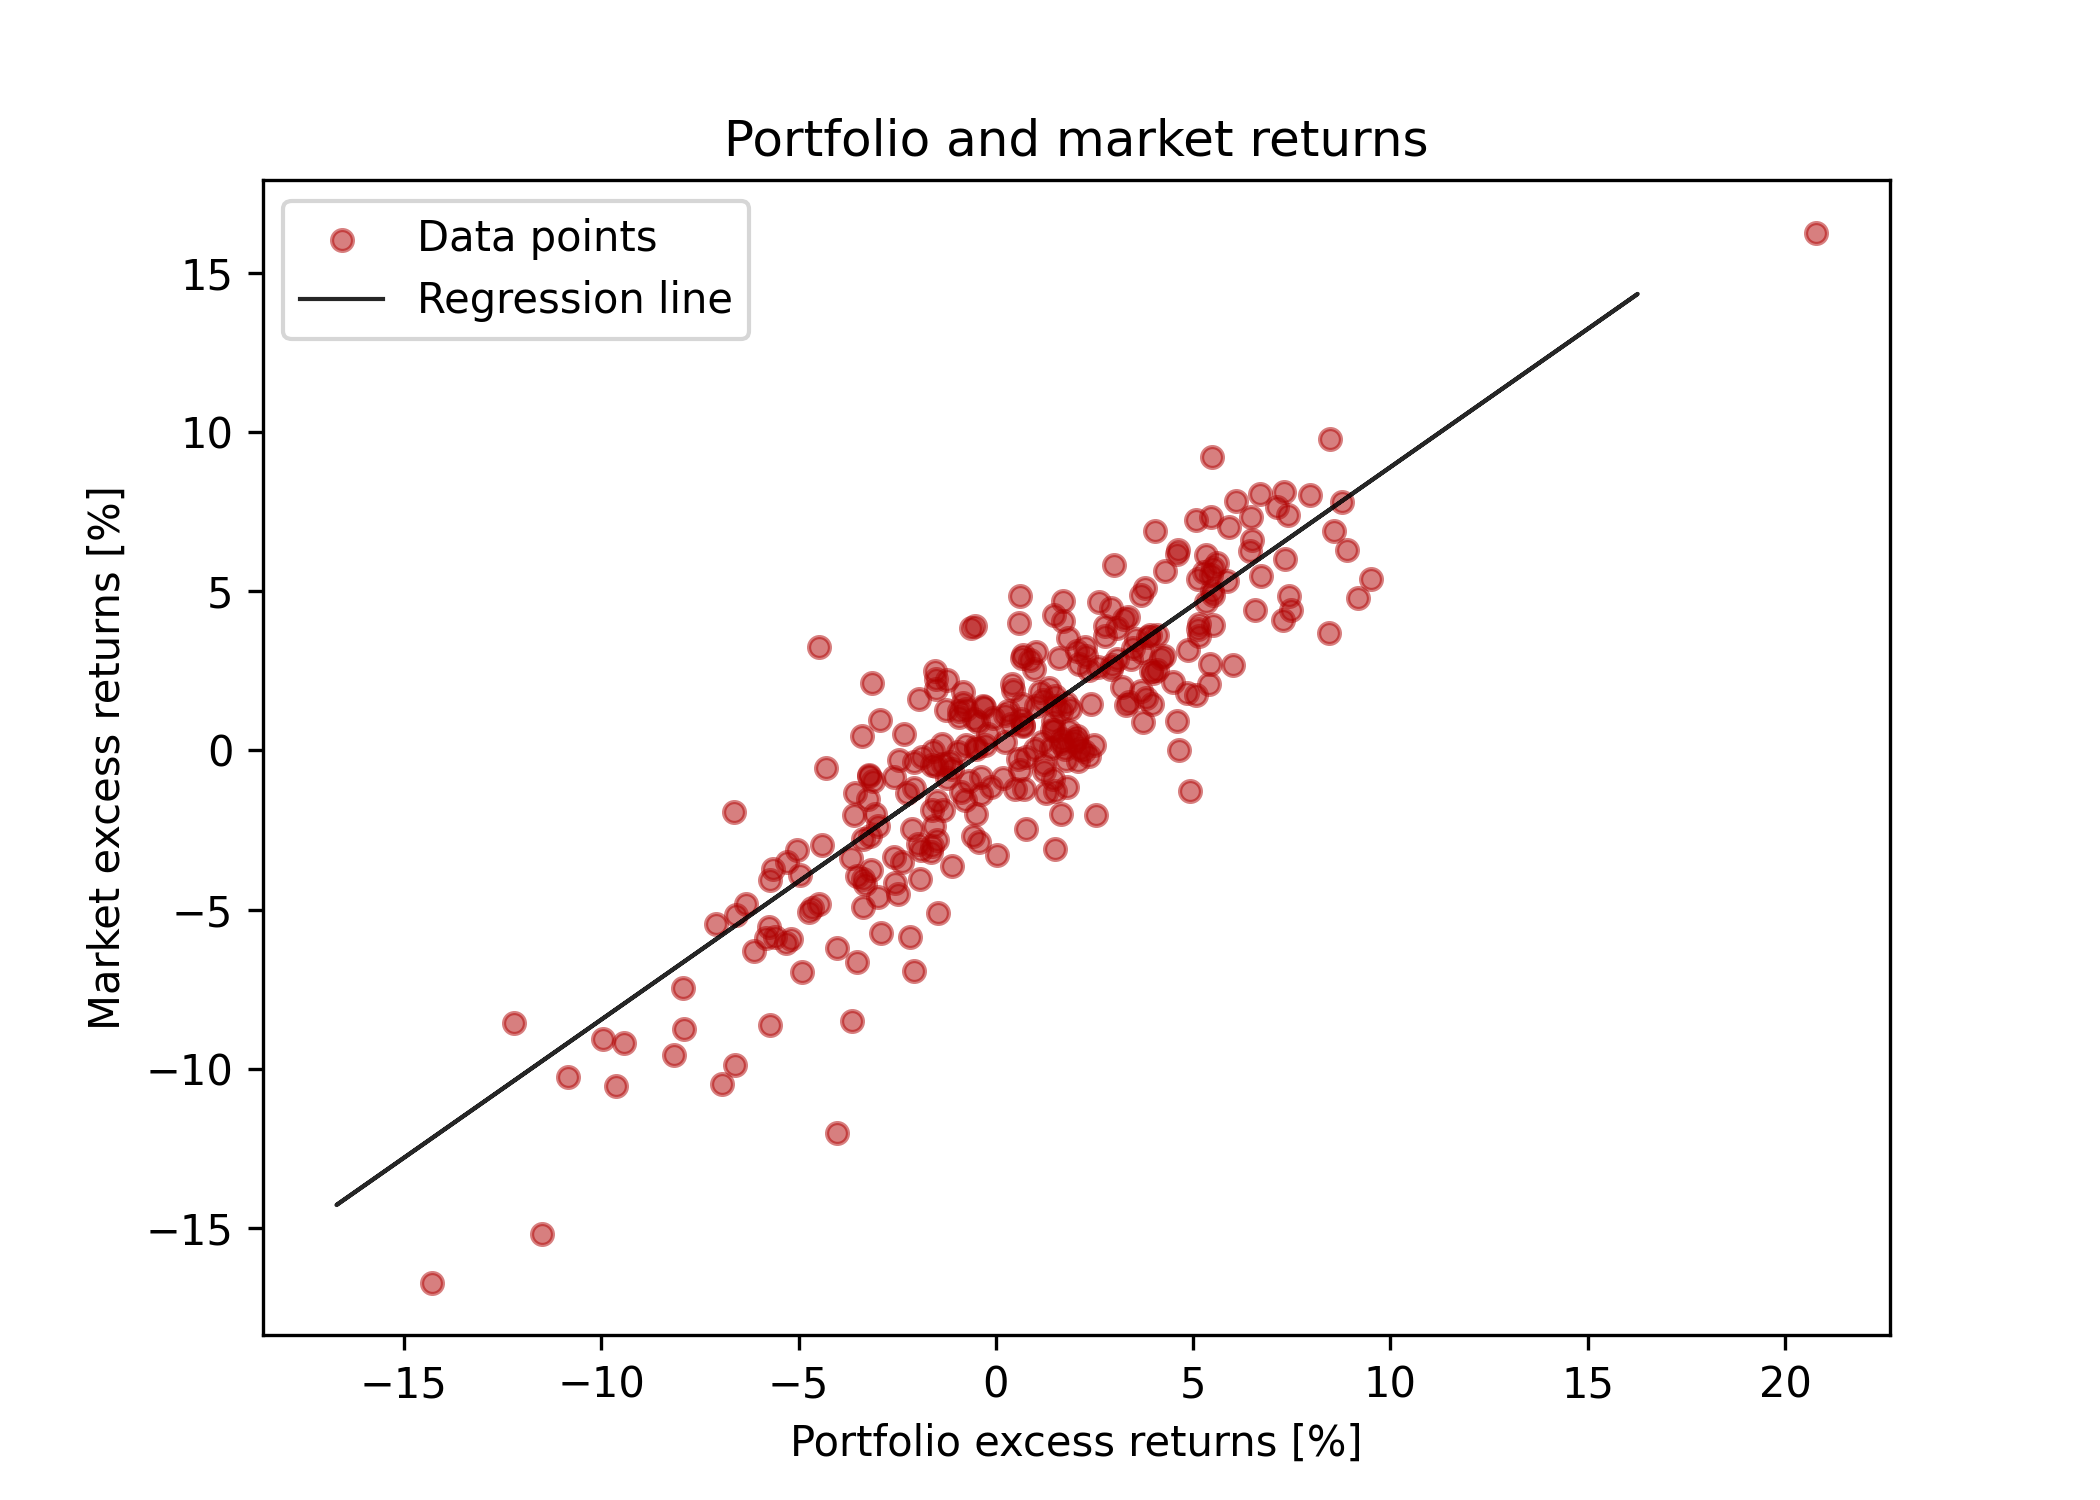
\includegraphics[width=0.9\textwidth]{images/portfolio_regression.png}
    \caption{Scatterplot of portfolio's returns against excess market returns, with linear regression.}\label{fig:portfolio_regression}
\end{figure}
%-------- Assignment 4 -----------------------------------------------------------------------------------------------------%
\section*{Assignment 4}
%-------- Assignment 5 -----------------------------------------------------------------------------------------------------%
\section*{Assignment 5}
\begin{figure}[h!]
    \centering
    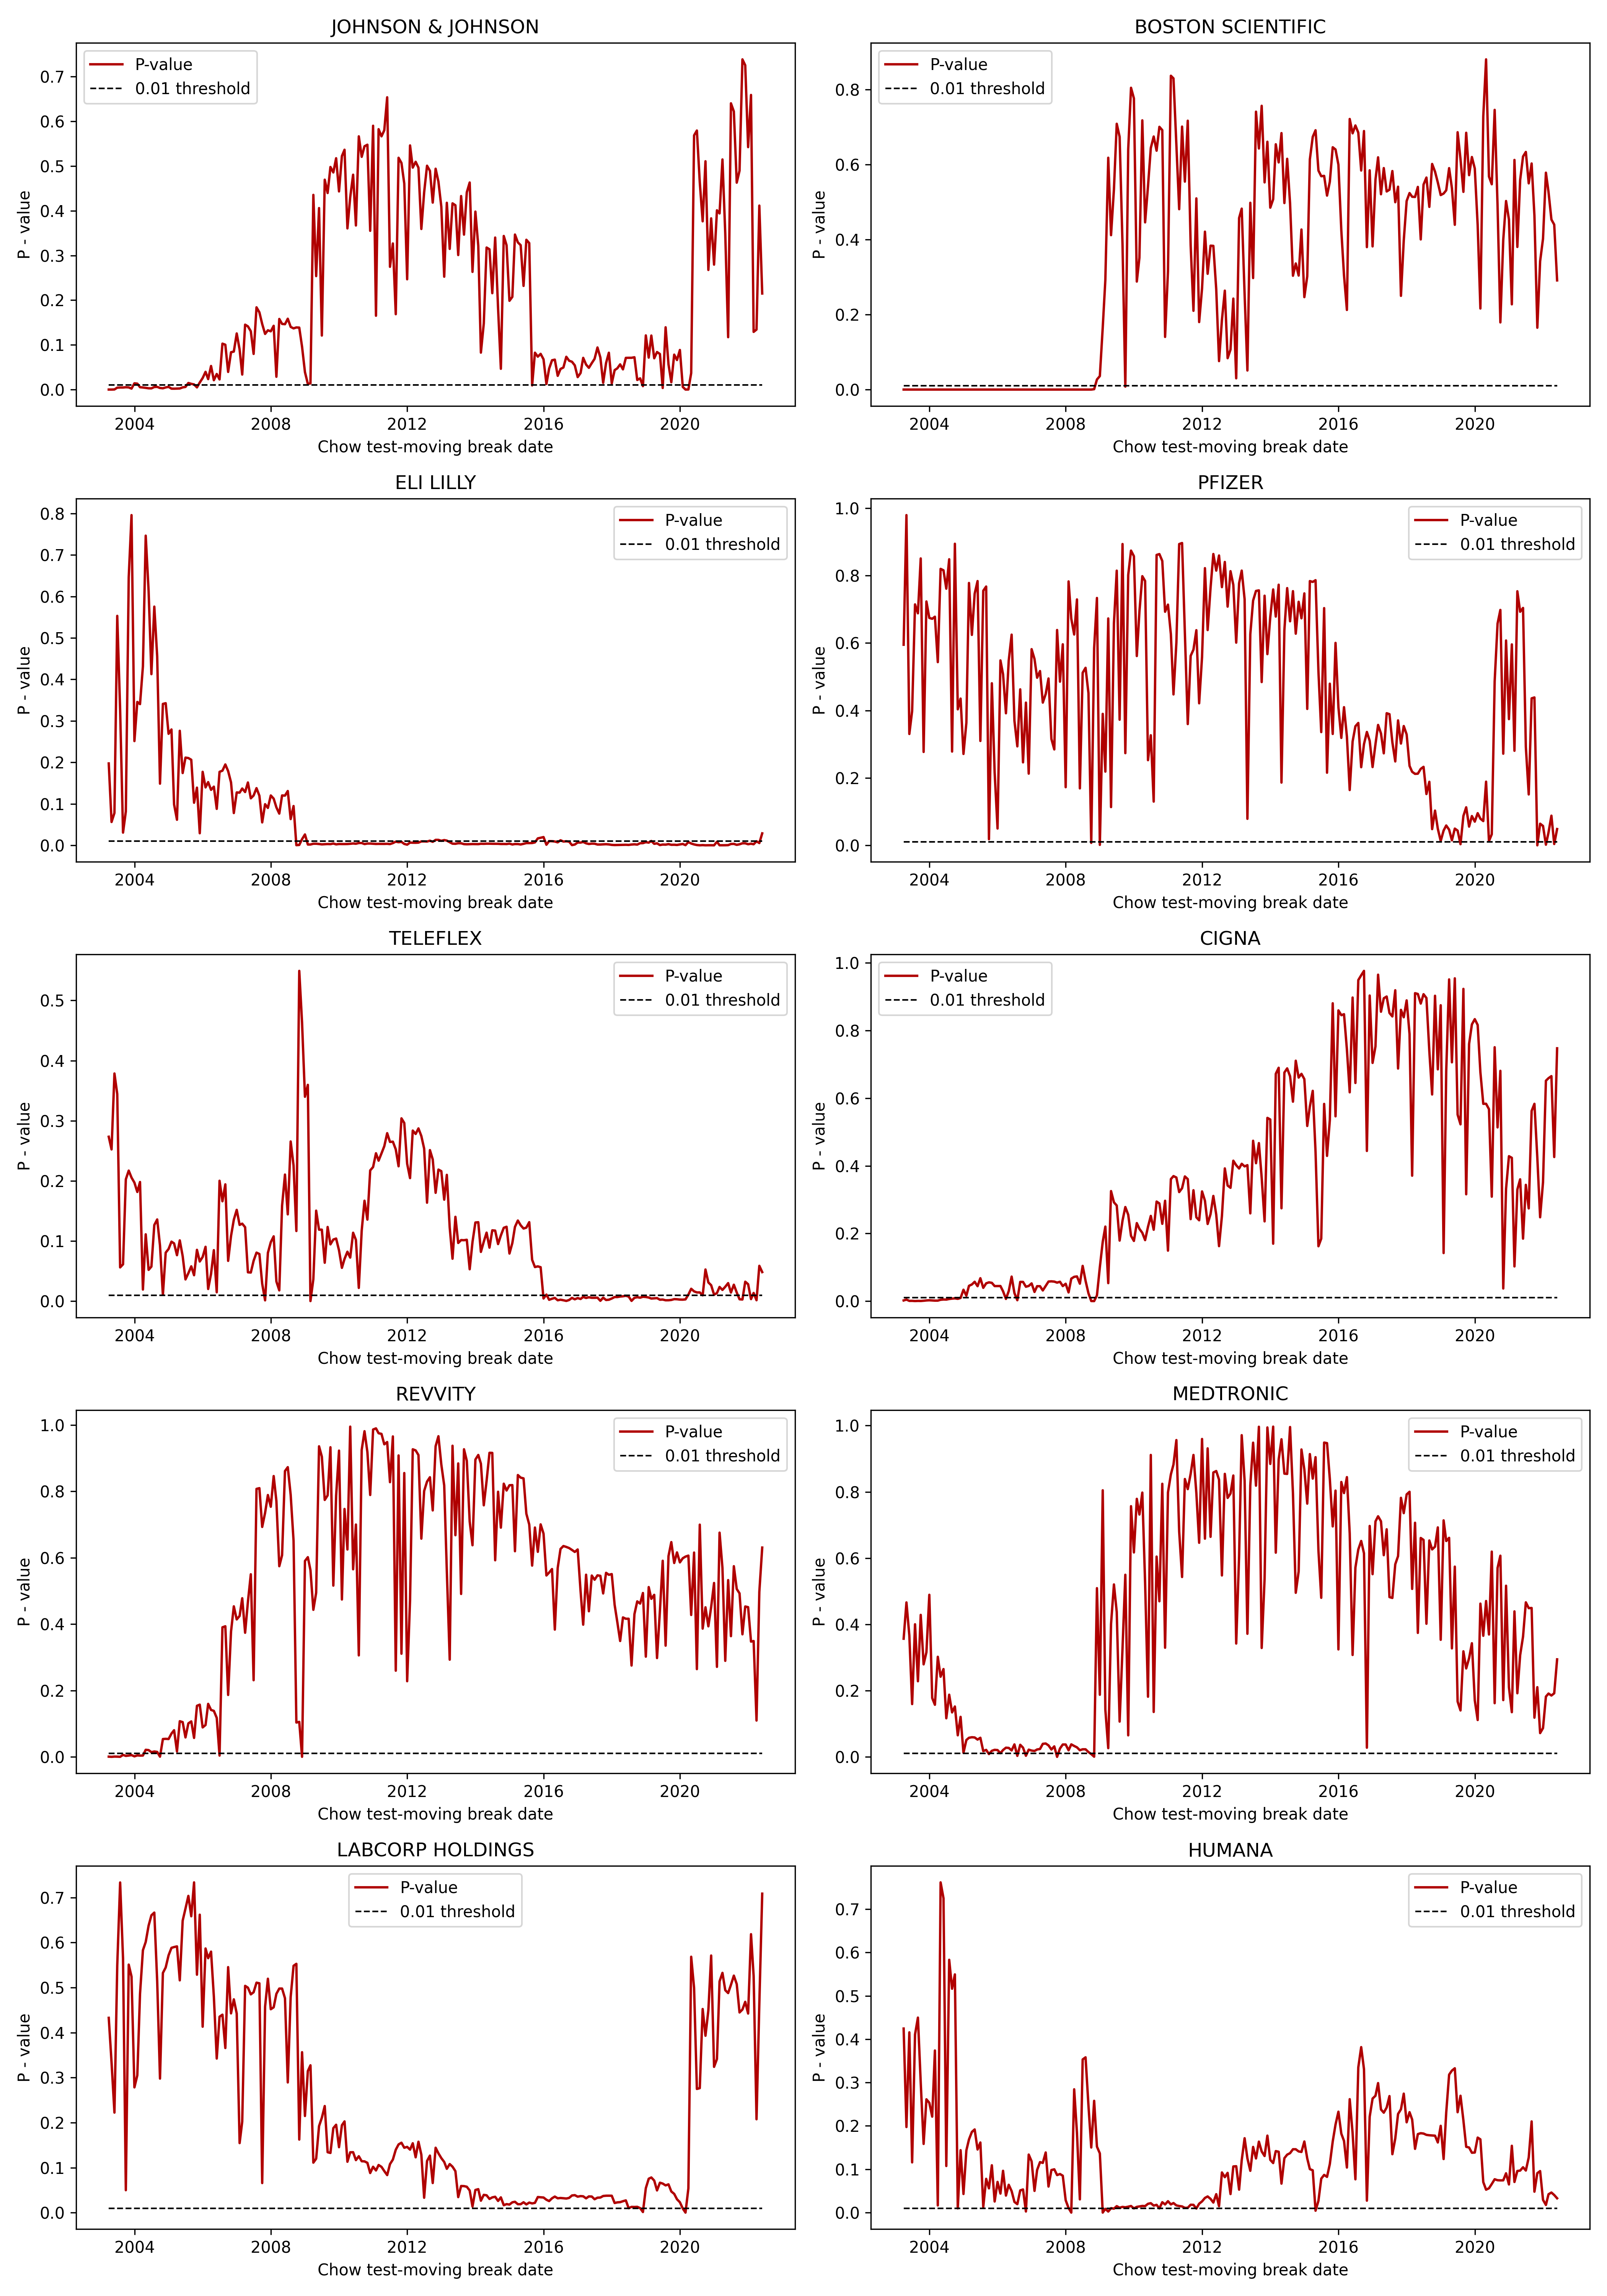
\includegraphics[width=0.9\textwidth]{images/chowmoving.png}
    \caption{Chow Test performed for all equities in search of structural breaks.}\label{fig:chowmoving}
\end{figure}
%-------- Assignment 6 -----------------------------------------------------------------------------------------------------%
\section*{Assignment 6}

\begin{figure}[h!]
    \centering
    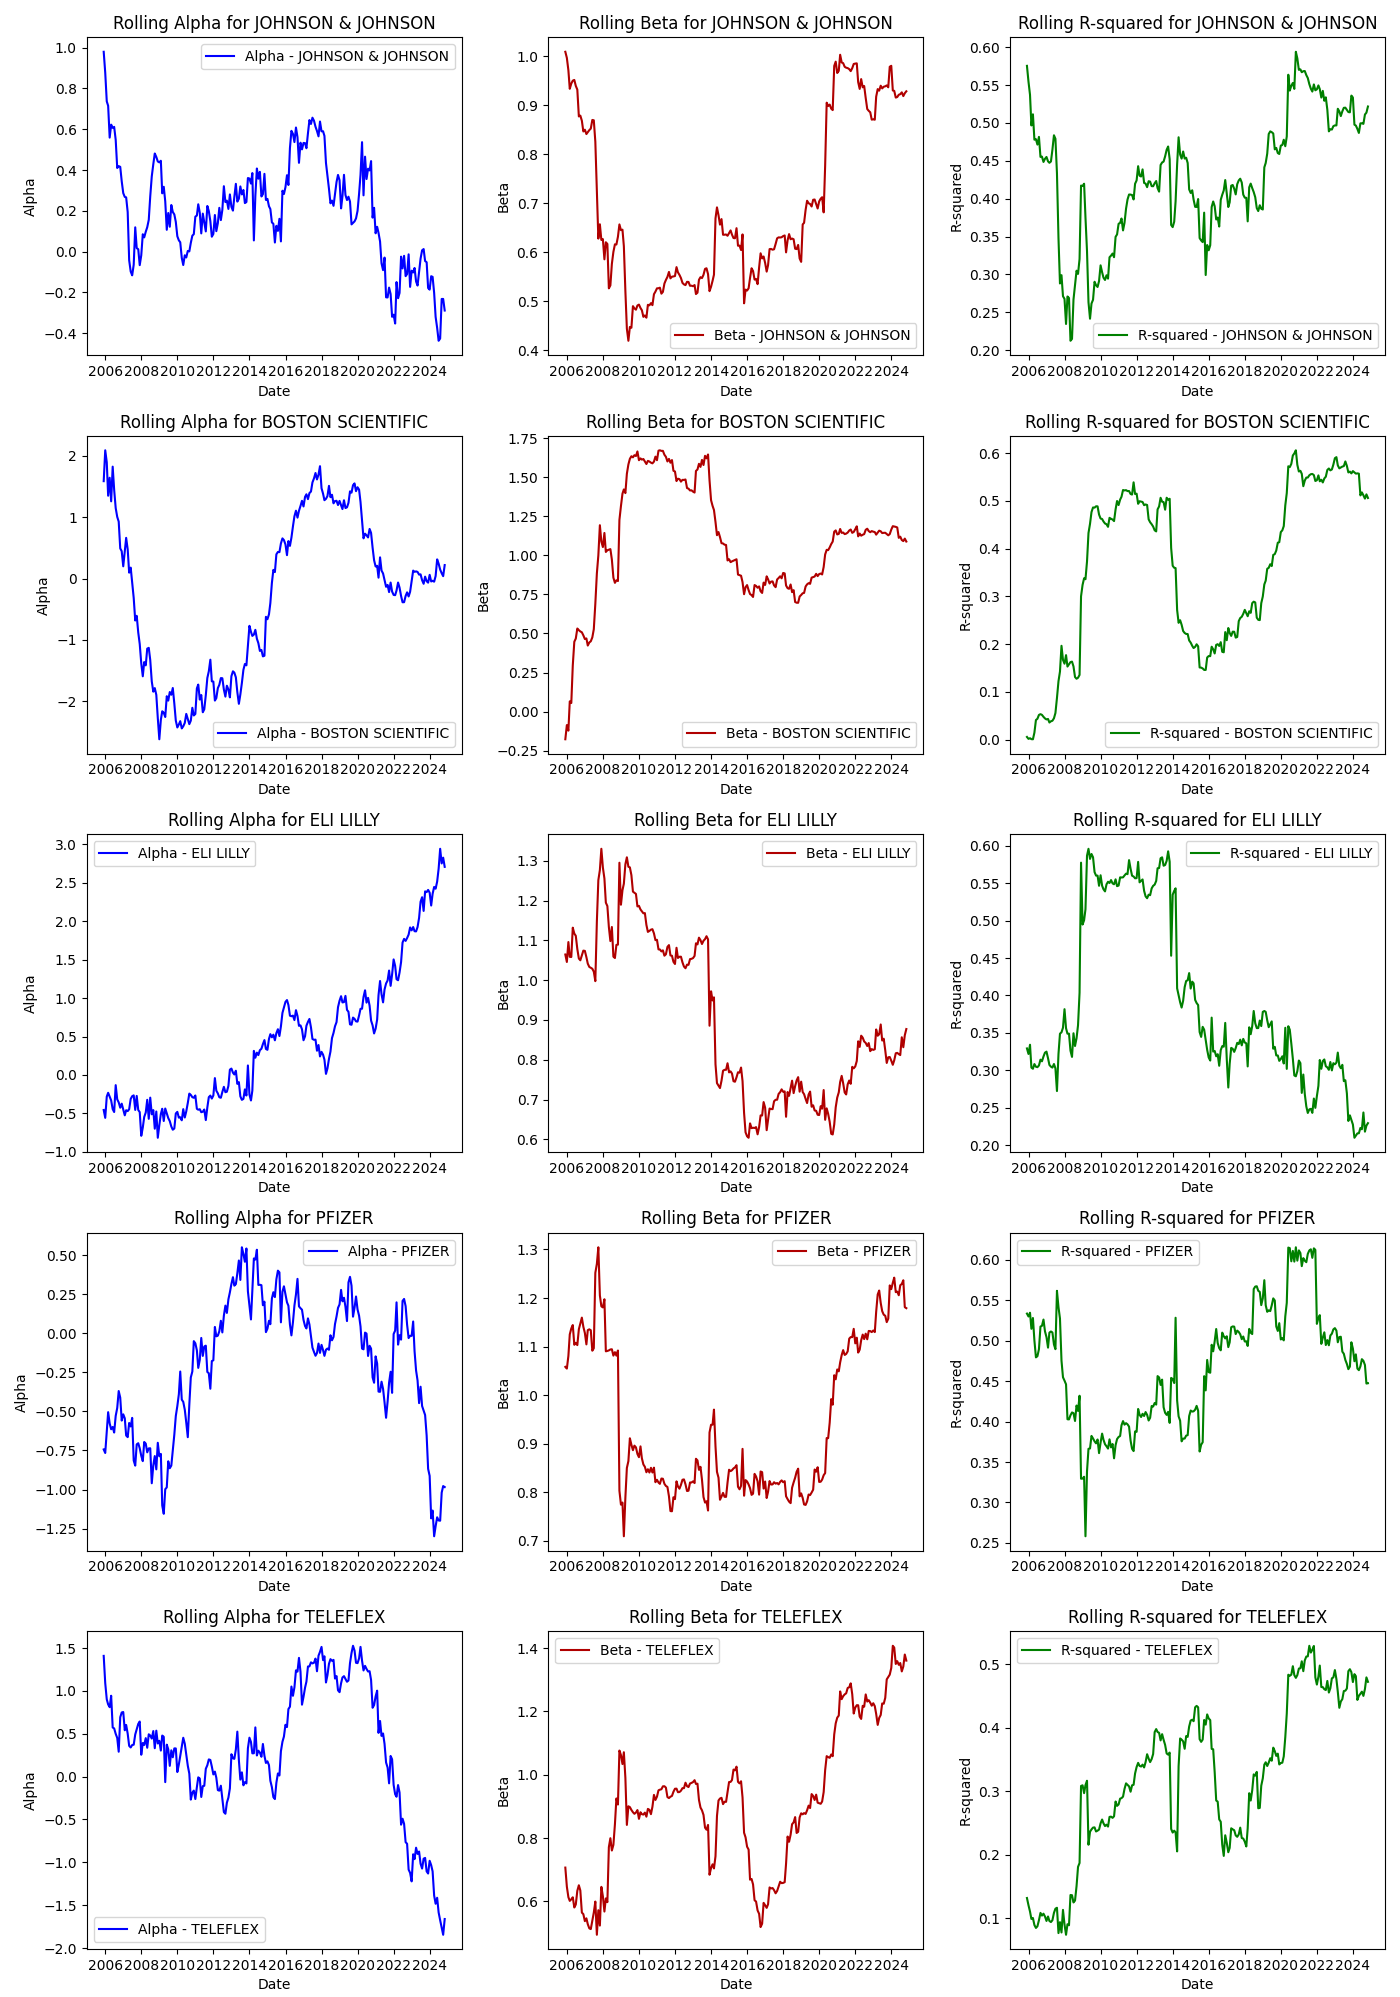
\includegraphics[width=0.9\textwidth]{images/rolling_quantities_1.png}
    \caption{Rolling quantities computed an all equities as an alternative of the Chow Test in search for structural
    breaks (1).}\label{fig:rolling_quantities_1}
\end{figure}
\begin{figure}[h!]
    \centering
    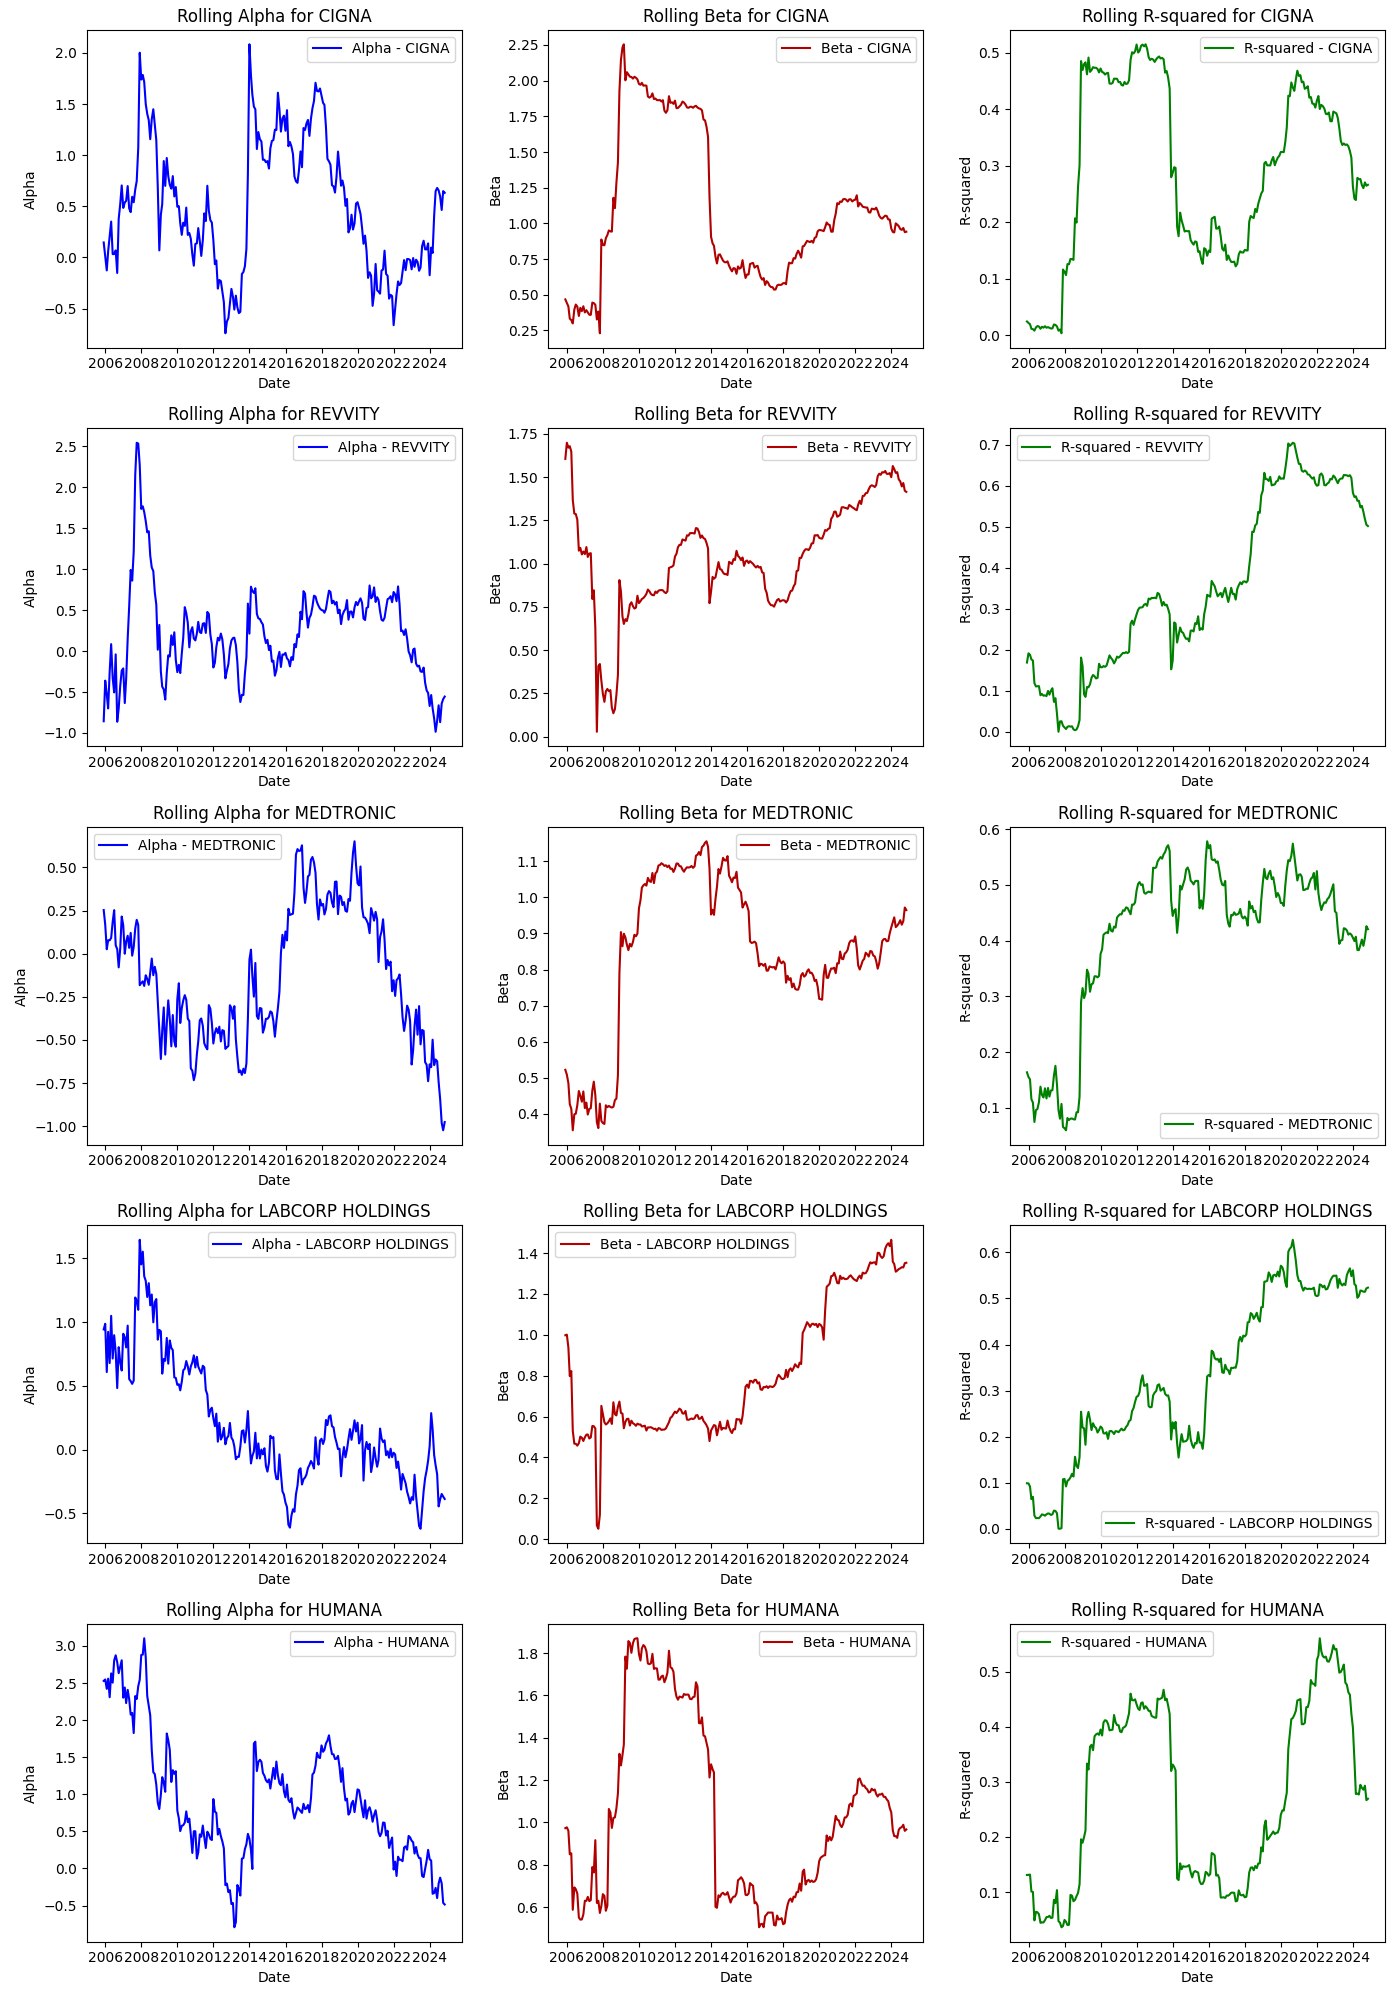
\includegraphics[width=0.9\textwidth]{images/rolling_quantities_2.png}
    \caption{Rolling quantities computed an all equities as an alternative of the Chow Test in search for structural
    breaks (2).}\label{fig:rolling_quantities_2}
\end{figure}

%-------- Assignment 7 -----------------------------------------------------------------------------------------------------%
\section*{Assignment 7}

\begin{figure}[h!]
    \centering
    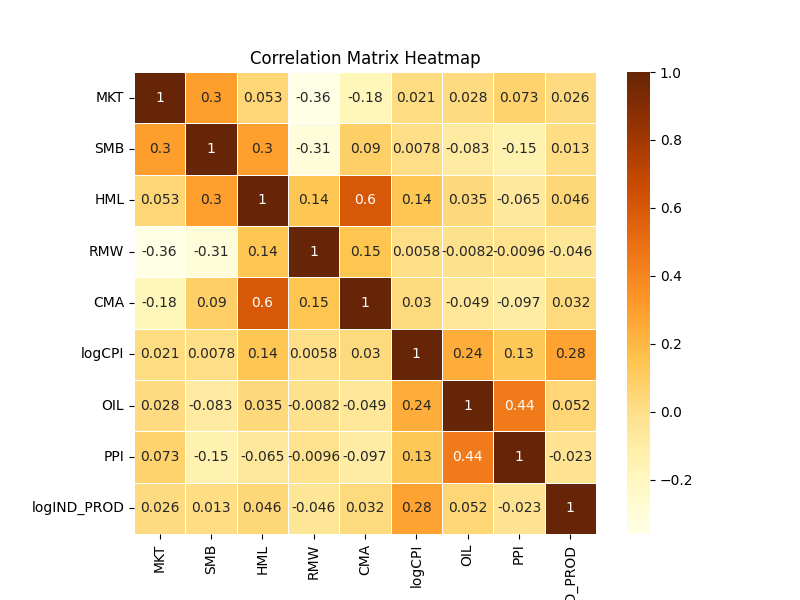
\includegraphics[width=0.9\textwidth]{images/Correlation_heatmap.png}
    \caption{Heatmap of the correlations between the chosen explainatory variables.}\label{fig:Correlation_heatmap}
\end{figure}
\end{document}

%-------- Appendix --------------------------------------------------------------------------------------------------------%
\section*{Appendix}